\documentclass[]{article}

%funny text
\usepackage[utf8]{inputenc} % set input encoding (not needed with XeLaTeX)
\usepackage[T1]{fontenc}
\DeclareUnicodeCharacter{00A0}{ }

%packages
\usepackage[english]{babel}
\usepackage[nottoc,notlof,notlot]{tocbibind} % Put the bibliography in the ToC
\usepackage{hyperref} % use hyperlinked ToC
\usepackage{parskip}
\usepackage{booktabs} % for much better looking tables
\usepackage{array} % for better arrays (eg matrices) in maths
\usepackage{paralist} % very flexible & customisable lists (eg. enumerate/itemize, etc.)
\usepackage{verbatim} % adds environment for commenting out blocks of text & for better verbatim
\usepackage{subfig} % make it possible to include more than one captioned figure/table in a single float
\usepackage{listings} %for code listings
\usepackage{color} %for colored syntax highligting
\usepackage{rotating}
\usepackage{pdflscape}
\usepackage[]{algorithm2e}
\usepackage{multirow}
\usepackage{float}
\usepackage{mathtools}
\usepackage{amssymb}
\usepackage{geometry} % to change the page dimensions
\usepackage{indentfirst}
\usepackage[printonlyused]{acronym}
\usepackage[backend=bibtex, bibencoding=utf8]{biblatex}

\graphicspath{ {assets/} }

\bibliography{biblib} 

%%% Page geometry
\geometry{a4paper} % or letterpaper (US) or a5paper or....
\geometry{margin=2.7cm}

%%% Paragraphs and text 
\setlength{\parindent}{4em}
\setlength{\parskip}{1em} 
\renewcommand{\baselinestretch}{1.3}
\setlength{\parskip}{10pt plus 1pt minus 1pt}

%%% Code listing
\definecolor{mygreen}{rgb}{0,0.6,0}
\definecolor{mygray}{rgb}{0.5,0.5,0.5}
\definecolor{mymauve}{rgb}{0.58,0,0.82}
\lstset{
basicstyle=\footnotesize\ttfamily,
commentstyle=\color{mygreen},
keywordstyle=\color{blue},
numberstyle=\tiny\color{mygray},
numbers=left,
tabsize=2,
frame=tb,
aboveskip=3mm,
belowskip=3mm,
breaklines=true,
breakatwhitespace=true,
showstringspaces=false,
columns=flexible
}
% to include a file as a listing: \lstinputlisting{intio.c}
% inline listing: \begin{lstlisting}[frame=single]

\hypersetup{colorlinks=true, linkcolor=black, citecolor=black, filecolor=black, urlcolor=black}

%%%%%%%%%%%%%%%%%%%%%%%%%%%%%%%%%%%%%%%%%%%%%%%%%
%%%%%%%%%%%%%%%%%%%%%%%%%%%%%%%%%%%%%%%%%%%%%%%%%

\title{A Wireless  Low Energy Ambulatory Electroencephalogram}
\author{Thomas Alexander Morrison (tm1810)}
\begin{document}

\maketitle

\begin{titlepage}
% \newgeometry{top=25mm,bottom=25mm,left=38mm,right=32mm}
\setlength{\parindent}{0pt}
\setlength{\parskip}{0pt}
% \fontfamily{phv}\selectfont

{
\Large
\raggedright
Imperial College London\\[17pt]
Department of Electrical and Electronic Engineering\\[17pt]
Final Year Project Report 2014\\[17pt]

}
\rule{\columnwidth}{3pt}

\vfill

\centering
% \includegraphics[width=0.7\columnwidth,height=60mm,keepaspectratio]{imgs/MyRobot.jpg}

\vfill

\setlength{\tabcolsep}{0pt}
\begin{tabular}{p{40mm}p{\dimexpr\columnwidth-40mm}}
Project Title: & \textbf{A Wireless  Low Energy Ambulatory Electroencephalogram} \\[12pt]
Student: & \textbf{Thomas Alexander Morrison} \\[12pt]
CID: & \textbf{00642176} \\[12pt]
Course: & \textbf{ISE4} \\[12pt]
Project Supervisor: & \textbf{James Mardell} \\[12pt]
Second Marker: & \textbf{Dr. Pants Georgiou} \\
\end{tabular}
\end{titlepage}

\clearpage





\clearpage

\section*{Abstract}
Certain neurological medical disorders require continuous monitoring to fully understand and diagnose. Examples of medical interest include epilepsy, syncope, multiple sclerosis, migraines, strokes, Parkinson’s and Alzheimer’s disease. \ac{EEG} is the recording of electrical activity along the scale, resulting from ionic current flows within the neurons of the brain and is useful for both diagnostic and monitoring such afromentioned conditions. Monitoring brain activity can help physicians understand certain characteristics, triggers, and the severity of the disorder. It may be possible to gauge the regions of the brain where the condition is originating from and if the patient is a suitable candidate for treatment. 
However, patients are unlikely to suffer from neurological disorders while at the clinic as they often appear sporadically during day to day life and with little to no warning. In such circumstances the patient could remain in hospital indefinitely, however seizures can be minutes to years apart, and sometimes are not realised or detected without proper equipment. Such circumstances lend themselves to an ambulatory system, where the patient can be monitored continuously without discomfort or hospitalisation, thus improving quality of life. 

With the emergence of low power wireless technologies coupled with portable devices such as tablets and phones, it is a natural technological step to bring care and monitoring out of the hospital and into the home. Through leveraging of low energy radio capable devices, i.e. smartphones and tablets, in the context of an ambulatory EEG, it is possible to empower the patient to inexpensively take health care into their own home and out of the hospital. Further, while this project is targeted at EEG signals, there is no reason why this research and technology cannot be applied to other signals and systems, for example glucose monitoring, electrocardiography, spirometers, etc.
\cite{Blanco95}
\clearpage
\tableofcontents
\clearpage

%Don't be gay
\section{Acknowledgements}
The opporunity is taken here to express gratitude to all those who have directly contributed towards the project. 

Firstly, the project surperivsors, James Mardell, Chen Guangwei and Esther Rodriguez-Villegas for their. 

Cambridge Silicon Radio providing hardware and technical support. Employees particurarly are Adam Hill, Martin Spikings, Mark Wade, Neil Stewart and Simon. The recently launched uEnergy forum is an excellent source of . CSR also await a report on the speed of 

Dr. Nissim Zur, CEO of Vitelix Limited is an expert in low power wireless technologies, and has conversed over many aspects of the final chip used. Further, has also taken an interest in this project's work in regards to maximising the speed, and has requested the results be shared with him.

Finally, and arguarbly most importantly Mike Harbour and Victor Boddy for their efforts in printed circuit board manufacture and assembly. Countless hours were spent in the lab pushing the department's PCB fabrication facilities outside their specifiction and to their limit. 

\clearpage

\section{Introduction}
Patients, however, are unlikely to suffer from neurological disorder while at the clinic as they often appear sporadically during day to day life and with little to no warning. In such circumstances the patient could remain in hospital indefinitely, however seizures can be minutes to years apart, and sometimes are not realised or detected without proper equipment. Such circumstances lend themselves to an ambulatory system, where the patient can be monitored continuously without discomfort or hospitalisation, thus improving quality of life. 



\subsection{Problem Landscape and Motivation}
Neurological disorders and their sequelae are currently estimated to affect upto one seventh of the world's population, a figure which currently stands at 1 billion. With the ever increasing life expectency and decreasing (relative) fertility rates, the population age demographic has shifted towards an ageing population. In tandem, the rates for neurological disorders has increased and is expected to increase further. Diagnosing, monitoring and treating many of these diseases is currently a costly procedure simply due to the time. 

Unfortunately many neurlogical disorder symptons occur sporadically with little to no inidication of an event, such a  in the cause of a seizure for epilepsy.



The vast majority of modern smart phones are now being equiped with \ac{BLE} or "Bluetooth Smart" technology. This is a relatively new technology design branded off the popular Bluetooth technology which gained popularity in the early part of last decade. While the two technologies share the same name, their design and operation is very much different. Although origianl Bluetooth's and \ac{BLE}'s use cases may overlap in some scenarios, they were designed to perform well under different circumstances.  

By coupling cheap low power sensors and radios, with powerful ubiquitous consumer technology, it is possible not only to cheaply and efficiently monitor patients, improve the quality of life for patients but also help physicians further their understanding of neurological disorders.

%Smart phone considered high power device anyway. Only hard requirement is that smart phone can support BLE
Currently \ac{BLE} is the only radio technology that is currently being built into all smart phones and tablet devices while offering power consumption low enough to enable a long lifetimes from a lightweight power source. In comparison classic Bluetooth’s power consumption is typically 1 to 2 orders of magnitude higher than BLE. Through leveraging widely popular and familiar smart phone devices with this new technology, in the context of an ambulatory EEG, it is possible to empower the patient to inexpensively take health care into their own home and out of the hospital.


\subsection{Existing Technologies and Products}


With the plethora of emerging low power wireless technologies coupled with portable devices such as tablets and phones, it is a natural technological step to bring care and monitoring out of the hospital and into the home. The consumer fitness sector is being targeted quite strongly, and many devices already exist that utilise lower power technologies to act as gateways for real-time data logging. For example, there already exists a competitive market between heartbeat monitors, cadence monitors and pedometers. These ‘activity trackers’ use low power electronics and radios to log user’s activities and update the user in real time with activity information through the user’s phone or smart watch. Popular products on the market at the time of writing include the Fitbit, Fuelband and Jawbone, which all use the \ac{BLE} technology to connect to smartphones.

\subsection{Project End Goals}
While the project goal is to make a wireless EEG device, the analouge front end will not be included. At the time of writing, the circuits and systems group at Imperial College have recently taped out a small full custom silicon design to a foundary. While it is possible . Originally the project was introduced as "Maximising Bluetooth Low Energy throughput of \ac{EEG} signals", however 

Currently, Imperial College has a wired EEG measurement device. The wired connection between the EEG sensors and a computer cause patients to remain fairly immobile and hence are impracticable for long periods of measurement. 

Hard requirements of the project include 
\begin{itemize}
	\item Running time of atleast 12 hours
	\item Channel resolution of 8 bits (albeit number of channels undefined)
	\item A weight of less than 10 grams
	\item 10 meter range
	\item BLE wireless technology
	\item Ability to communicate with a smart phone or tablet
\end{itemize}

\subsection {Structure}

\clearpage
\section{Theory and Technology}
\subsection{Bluetooth Low Energy}
The original Bluetooth, hereforth refered to a \ac{BTC}, was intially concieved as the solution to wired communication over short distances (typically less than 100m). The original specification had an air over-the-air rate of 1MBps, though this has increased to around 3 MBps in the latest version of \ac{BTC}. Similarly, BLE has an over-the-air rate of 1MBps. Despite the odd realisation that \ac{BLE}, a much newer technology, has the same over the air rate of last the first incarnation of \ac{BTC}, the maximum theoretical throughput of \ac{BTC} is 700kBps, compared to less than 250kBps for \ac{BLE} - roughly one third of the maximum throughput \ac{BTC} was capable of (the latest version of \ac{BTC} brings the disparity to one ninth). While intuatively it may seem that \ac{BLE} is a less efficient technology, \ac{BLE} can be orders of magnitudes more efficient than \ac{BTC} in particular use cases.

Applications where \ac{BLE} excels in are ones where communication between two devices is only required intermitently, and the volume of information sent is small. An example would be a thermometer in a green house connected by radio to a visual display unit inside the home. Temperature changes at a rate slow enough that it is only necessary to check the temperature every 10 minutes. Once every 10 minutes the radio thermometer device can wake up take a measurement, send a notification of a measurement then return to a deep sleep. \ac{BLE} does this much better than \ac{BTC}, taking only a few milliseconds to connect. \ac{BTC} takes between a few hundred milliseconds to several seconds to reconnect. While both millisecond orders of magnitude and second orders of magnitude are small when compared to an order of magnitude of minutes, over time it adds up to a significant amount, and \ac{BLE} devices can last many years of a small, single coin cell. \ac{BLE} is excellent for applications which involve small episodic transmission of data. In the scenario described a \ac{BTC} system would have a lifetime of approximately 100 days from a typical 3v lithium cell. Off the same cell, a \ac{BLE} system would have a lifetime of many years.

There are more reasons 


Further, the reduced compelxity of \ac{BLE} means reduced memory requirements, in turn reducing the leakage current. Combined with also a 

Bluetooth was designed with the idea that it would be used to do many common jobs, and hence particular configurations were built into it. In Bluetooth, these configurations are known as profiles. Example profiles include the audio distribution profile (A2DP), which is used in by many Bluetooth product manufacturers to allow a device, such as a phone to interact with an audio system, such as in a car. Another example would be the serial port profile (SPP), meant to emulate the highly popular and robust RS-232 (serial) standard for data transfer. This is all built into what is known as the Bluetooth stack – a software framework that interacts between the physical layer and the application layer.  

BLE borrows many of these concepts and features and it is often mistakenly thought of as \ac{BTC} operating at lower speeds and power consumption. It is not currently compatible with Bluetooth and there are no plans for it to be. As mentioned, \ac{BLE} has a maximum application throughput of roughly one third that of the \ac{BTC} version 1.0. There are many reasons for this, but all ultimately converge on power. BLE was designed to be simple, with a ‘less is more’ approach and if things are simple they can be done using less hardware, and ultimately less power. Like \ac{BTC}, the \ac{BLE} architecture has 3 over-arching parts: Application, Host and Controller. The controller, simply put, is the radio and the application the use case, which could be a cadence monitor, thermometer or even an electroencephalogram. It is the host controller interface (HCI), commonly known as the “stack” that provides the necessary software to enable the application layer to communicate with the radio (see Figure~\ref{fig:ble_arch}).


\begin{figure}[htb]
	\begin{center}
		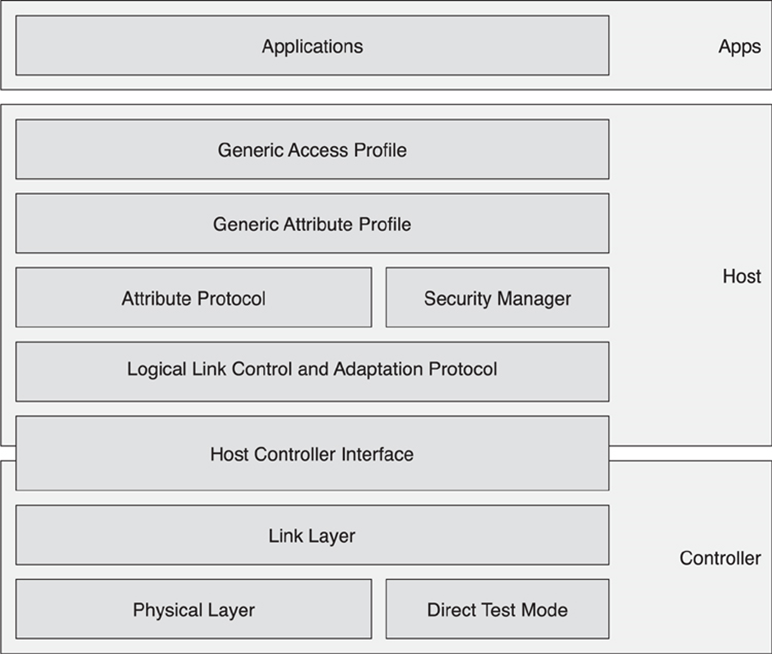
\includegraphics[width = 0.7\textwidth]{ble_arch}
	\end{center}
	\caption{\ac{BLE} Architecture}
	\label{fig:ble_arch}
\end{figure}

In an attempt to be economical with time and space components of the stack deemed irrelevant will not be discussed further here. For example a description of the security manager is not relevant as this project is not concerned with sending data over encrypted links. Similarly, the Logical Link Control and Adaption Protocol, while used extenivesly in communication will not be discussed in detail as it 

\ac{BLE}'s profiles are all built ontop of from the \ac{GATT}, which in turn is built upon the \ac{ATT}, a protocol optimised to run on BLE devices. Like in Bluetooth there are profiles, but these profiles are on a much smaller scale. The profiles arn't complex enough to warrant tailoring a microchiptowards a particular profile, unlike \ac{BTC}, whereby chips would be specifically designed to excel in one profile (i.e. A2DP). Popular examples of \ac{BLE} profiles include the heart rate profile (HRP), health thermometer profile (HTP) and even a glucose profile (GLP) with room for many more to be incorporated into the core \ac{BLE} specification. 

In BLE and BTC, there certain states the device. The same abstract view can be applied to both technologies and is shown in Figure 3. Note that depending on the role of the device, the state moves right (master) or left (slave) from standby. It may appearing confusing to have another state for scanning which can only move into the standby state, but this is useful for just searching and discovering devices with no commitment to connecting. 

In BLE the low power device is known as the peripheral (e.g. a cadence meter) and the master is the higher power device (e.g. a smartphone) . Assuming that the master BLE device is in the initiating state, searching for a device to make connection with, and at the same time the BLE slave is in the advertising stage, periodically broadcasting information using advertisement packets the two devices will find one another and may initiate a connection request.

In classic Bluetooth there are 79 channels, all of which could be used to both transmit data and advertise. BLE uses only 40 channels, and segments 3 channels for advertisement and the remaining 37 channel for data. Figure 4 show this. By only have 3 channels, a BLE slave will only have to broadcast on these few channels (and equally the master will only have to listen on these 3), saving power while decreasing connection latency. 

\section{Radio Evaluation}

\section{Prototype Design}

\section{Results}

\section{Evaluation}

\subsection{Power Analysis}

\subsection{Bill of materials}

\section{Conclusions and Future Work}
On the whole, the project has 

Not all tablets will be able to run at full speed

Ideally, it is desirable to write a conference style paper. 

Useful for CSR
\section{Final Remarks}
A vast array of technologies and tools were used throughout this project. Below highlights those that are non-trivial and were of significant importance

\begin{itemize}
	\item Git verisioning control - For versioning and segmenting the workflow
	\item xIDE - CSRs integrated development suite for compiling and debugging CSR-stack based chips. This is where the firmware for the CSR1010 MCU was written
	\item Wireshark - Invaluable in analysing the packets and control flow between BLE radios, unfortunately must be used offline
	\item SmartRF online packet sniffer - Useful as a low-speed packet sniffer. Extremely useful in the early days of the project, however the throughputs eventually obtained rendered the tool and hardware redundant as it was not capable of such speeds
	\item Visual Studio 2013 - Primairly used for developing the tablet application. Highly useful for "knocking up" quick throughput expirements 
\end{itemize}

The large amount of both written and generated code is to vast to warrant being included in this report. Therefore is has been decided to make it publically available online at the git repositry address 
\url{https://github.com/proftom/AmbulatoryEEG}.

\section{Bibliography}
\clearpage

\nocite{*}

\printbibliography


\section{Appendix}
\subsection{Acronyms}
\begin{acronym}
	\acro{EEG}{Electroencephalography}
	\acro{BLE}{Bluetooth Low Energy}
	\acro{BTC}{Bluetooth Classic}
	\acro{CSR}{Cambridge Silicon Radio}
	\acro{GATT}{Generic Attribute Prorfile}
	\acro{GAP}{Generic Access Profile}
	\acro{ATT}{Attribute Protocol}
\end{acronym}

\section{User Guide}
\end{document}